% Tích hợp nội dung từ Chuong3.pdf. Mã và ngưỡng giữ theo nguồn trừ phần AI bổ sung.
\section{Phân tích và đặc tả yêu cầu}
\label{sec:requirements}
\begingroup
\setstretch{1.12}
\setlength{\parskip}{4pt}
\renewcommand{\arraystretch}{1.22}
\setlength{\extrarowheight}{1pt}

\subsection{Tác nhân và nhóm chức năng}
CultureMap VN có ba tác nhân. Khách truy cập nội dung công khai. Thành viên đã đăng nhập
có thể gửi đóng góp và báo cáo sai lệch. Quản trị viên chuẩn bị dữ liệu, kiểm chứng nguồn,
xử lý yêu cầu và quản lý kho nội dung. Quyền kiểm chứng thuộc quản trị viên.


\begin{longtable}{|L{28mm}|L{116mm}|}
\caption{Tác nhân và trách nhiệm chính}\label{tab:actors}\\\hline
\rowcolor{gray!15}\textbf{Tác nhân} & \textbf{Nhóm chức năng}\\\hline
\endfirsthead
\hline
\rowcolor{gray!15}\textbf{Tác nhân} & \textbf{Nhóm chức năng}\\\hline
\endhead
\endfoot
Khách vãng lai & Xem bản đồ, chọn hoặc tìm tỉnh/thành, duyệt danh mục, đọc bài và nguồn. Hỏi thêm về bài bằng RAG. Có thể đăng ký tài khoản thành viên.\\\hline
Thành viên & Có các chức năng khám phá của khách. Gửi đề xuất bài mới, báo cáo thông tin sai hoặc lỗi thời, theo dõi trạng thái và kết quả xử lý.\\\hline
Quản trị viên & Quản lý bài, nguồn và dữ liệu ban đầu. Kiểm chứng đóng góp và báo cáo, quản lý phiên bản, nhật ký và trạng thái tài khoản thành viên.\\\hline
\end{longtable}

Nhóm phát triển xây dựng, triển khai và bảo trì hệ thống. Đơn vị phát hành tài liệu
tham khảo cung cấp nguồn được trích dẫn trong quá trình biên soạn và đối chiếu.

\subsection{Phạm vi chức năng được chọn để hiện thực}
Trong phạm vi đồ án, hệ thống tập trung vào khám phá tri thức địa phương và kiểm chứng
nội dung. Phần AI gồm hỏi đáp bằng RAG trên tư liệu của bài và thử nghiệm fine-tuning
quy mô nhỏ trên một nhiệm vụ liên quan đến sản phẩm.

\subsubsection{Phạm vi địa lý và nội dung}
Bản đồ Việt Nam giúp người dùng định hướng theo ba miền Bắc, Trung và Nam. Dữ liệu dự
kiến bao phủ khoảng 3--5 tỉnh/thành đại diện ba miền. Tỉnh ngoài phạm vi vẫn xuất hiện
trên bản đồ nền ở trạng thái bất hoạt. Kết quả tìm kiếm địa phương có thể thông báo
khi tỉnh người dùng cần tìm chưa được hỗ trợ.

Nội dung gồm ẩm thực và đặc sản, danh lam thắng cảnh và địa danh, lễ hội và sự kiện văn hóa,
nghề và làng nghề, phong tục và tập quán. Mỗi bài gắn với một địa phương và một danh mục
chính. Vị trí, lịch sử, thời gian tổ chức, hình ảnh và thuộc tính chuyên biệt được thêm
tùy loại nội dung. Nhóm thực hiện chuẩn bị dữ liệu ban đầu từ nguồn có xuất xứ rõ ràng.

\subsubsection{Khám phá tri thức}
\begin{enumerate}
  \item Người dùng xem bản đồ để nhận biết các địa phương có dữ liệu khám phá.
  \item Người dùng chọn một tỉnh/thành đang tương tác hoặc tìm tỉnh/thành theo tên.
  \item Hệ thống hiển thị các danh mục đã có bài công khai ở địa phương đó.
  \item Người dùng chọn danh mục, duyệt danh sách và mở bài cần tìm hiểu.
  \item Trang chi tiết hiển thị nội dung, thuộc tính theo danh mục, hình ảnh, vị trí nếu có,
        nguồn tham khảo và thời điểm cập nhật.
\end{enumerate}
\subsubsection{Đóng góp và kiểm chứng tri thức}
\ReportBlockHeading{Đóng góp tri thức mới}
Thành viên gửi địa phương, danh mục, tiêu đề, nội dung, nguồn hoặc minh chứng và hình ảnh
nếu có. Hệ thống kiểm tra dữ liệu và lưu yêu cầu chờ xử lý. Admin đối chiếu nguồn, kiểm tra
mức độ phù hợp và khả năng trùng lặp. Khi duyệt, hệ thống tạo tri thức chính thức, phiên bản
đầu tiên và liên kết nguồn. Nếu từ chối, admin ghi lý do để thành viên xem lại.

\ReportBlockHeading{Báo cáo bài sai hoặc lỗi thời}
Thành viên báo cáo trên trang chi tiết bài, nêu sai lệch, minh chứng và đề xuất sửa nếu có.
Báo cáo gắn với cả bài và phiên bản đã xem. Admin đối chiếu nguồn, phiên bản bị báo cáo và
lịch sử sửa đổi. Báo cáo có cơ sở được chấp nhận để soạn bản sửa. Sau khi bản sửa được công
bố, hệ thống ghi nhận khắc phục hoàn tất. Nếu báo cáo bị từ chối, người gửi nhận lý do.
Trạng thái công khai của bài do admin quyết định qua nghiệp vụ quản trị.

\subsubsection{AI hỗ trợ tìm hiểu văn hóa}
Khách hoặc thành viên hỏi thêm trên trang bài đọc. RAG truy xuất tư liệu đã kiểm chứng của
phiên bản đang công khai và đưa nguồn đi cùng câu trả lời. Fine-tuning được thực hiện ở quy mô
nhỏ trên mô hình có sẵn, được đánh giá trên nhiệm vụ đã chọn. Phương án và cách đánh giá
được trình bày tại Chương~\ref{sec:ai} và Chương~\ref{sec:evaluation}.

\subsubsection{Giới hạn phạm vi}
Đặt tour, đặt vé, thanh toán, chỉ đường, mạng xã hội, nhắn tin cá nhân và đánh giá sao
nằm ngoài phạm vi. Chỉ admin có quyền công bố hoặc sửa nội dung chính thức. Lưu yêu thích,
cá nhân hóa và lập kế hoạch trải nghiệm là các chức năng tùy chọn.

\subsection{Yêu cầu chức năng (FR)}
Mã FR liên kết hành vi của hệ thống với use case, thiết kế dữ liệu và ca kiểm thử.


\ReportNeedSpace{48mm}
\subsubsection{Khám phá tri thức}

\begin{longtable}{|L{20mm}|L{124mm}|}
\caption{Yêu cầu chức năng nhóm khám phá tri thức}\label{tab:chapter3-fr-1}\\\hline
\rowcolor{gray!15}\textbf{Mã} & \textbf{Nội dung yêu cầu}\\\hline
\endfirsthead
\hline
\rowcolor{gray!15}\textbf{Mã} & \textbf{Nội dung yêu cầu}\\\hline
\endhead
\endfoot
FR-01 & Hệ thống hiển thị bản đồ Việt Nam và phân biệt tỉnh/thành có dữ liệu khám phá. Tỉnh ngoài phạm vi hiển thị trên bản đồ nền, không đổi màu khi rê chuột và không nhận thao tác chọn.\\\hline
FR-02 & Người dùng chọn trực tiếp tỉnh/thành có dữ liệu trên bản đồ để bắt đầu khám phá.\\\hline
FR-03 & Người dùng có thể tìm tỉnh/thành theo tên, hỗ trợ tìm kiếm không dấu và hiển thị các kết quả phù hợp.\\\hline
FR-04 & Sau khi chọn một tỉnh/thành có dữ liệu, hệ thống hiển thị các danh mục tri thức đang được công bố tại tỉnh/thành đó.\\\hline
FR-05 & Hệ thống cho phép xem và lọc danh sách tri thức đang công bố theo tỉnh/thành và danh mục đã chọn.\\\hline
FR-06 & Hệ thống cho phép tìm kiếm tri thức đã công bố theo tiêu đề hoặc từ khóa. Có thể kết hợp với bộ lọc địa phương và danh mục.\\\hline
FR-07 & Hệ thống thông báo khi tìm một địa phương chưa hỗ trợ, khi danh mục trống hoặc khi tìm kiếm không có kết quả.\\\hline
FR-08 & Người dùng có thể xem chi tiết một tri thức gồm tiêu đề, tóm tắt, nội dung, thông tin đặc thù theo danh mục, hình ảnh, vị trí nếu có và thời điểm cập nhật.\\\hline
FR-09 & Người dùng có thể xem thông tin nhận diện các nguồn hỗ trợ phiên bản tri thức đang đọc và mở URL đối với nguồn trực tuyến có đường dẫn được công bố.\\\hline
\end{longtable}

\ReportNeedSpace{48mm}
\subsubsection{Tài khoản, đóng góp và báo cáo tri thức}

\begin{longtable}{|L{20mm}|L{124mm}|}
\caption{Yêu cầu chức năng nhóm tài khoản, đóng góp và báo cáo}\label{tab:chapter3-fr-10}\\\hline
\rowcolor{gray!15}\textbf{Mã} & \textbf{Nội dung yêu cầu}\\\hline
\endfirsthead
\hline
\rowcolor{gray!15}\textbf{Mã} & \textbf{Nội dung yêu cầu}\\\hline
\endhead
\endfoot
FR-10 & Hệ thống hỗ trợ đăng ký tài khoản thành viên, đăng nhập, đăng xuất và xác thực phiên của thành viên và quản trị viên. Quyền quản trị được cấp riêng.\\\hline
FR-11 & Thành viên đã xác thực có thể tạo yêu cầu đóng góp với địa phương, danh mục, tiêu đề, nội dung và ít nhất một nguồn hoặc minh chứng.\\\hline
FR-12 & Hệ thống cho phép đính kèm tối đa 5 ảnh JPEG/PNG/WebP, mỗi ảnh không quá 5 MB, kèm thông tin xuất xứ khi đóng góp. Các giới hạn tương tự áp dụng cho ảnh minh chứng báo cáo.\\\hline
FR-13 & Khi gửi đóng góp, hệ thống kiểm tra trường bắt buộc, nguồn/minh chứng và tệp đính kèm. Dữ liệu sai phải trả thông báo cụ thể và giữ biểu mẫu để chỉnh sửa. Dữ liệu hợp lệ tạo yêu cầu PENDING.\\\hline
FR-14 & Thành viên đã xác thực có thể báo cáo thông tin sai hoặc lỗi thời của tri thức đã công bố, kèm loại sai lệch, mô tả và minh chứng. Hệ thống ghi nhận mã tri thức và mã phiên bản thành viên đang xem.\\\hline
FR-15 & Khi gửi báo cáo, hệ thống kiểm tra mô tả, minh chứng và đối tượng bị báo cáo. Chỉ tạo báo cáo PENDING khi dữ liệu hợp lệ, nếu không thì trả lỗi.\\\hline
FR-16 & Thành viên có thể xem danh sách đóng góp và báo cáo của chính mình, trạng thái xử lý, lý do từ chối và kết quả giải quyết (nếu có).\\\hline
\end{longtable}

\ReportNeedSpace{48mm}
\subsubsection{Quản trị và kiểm chứng}

\begin{longtable}{|L{20mm}|L{124mm}|}
\caption{Yêu cầu chức năng nhóm quản trị và kiểm chứng}\label{tab:chapter3-fr-17}\\\hline
\rowcolor{gray!15}\textbf{Mã} & \textbf{Nội dung yêu cầu}\\\hline
\endfirsthead
\hline
\rowcolor{gray!15}\textbf{Mã} & \textbf{Nội dung yêu cầu}\\\hline
\endhead
\endfoot
FR-17 & Admin có thể xem, tìm kiếm, lọc hàng đợi đóng góp và báo cáo theo loại, trạng thái và thời điểm gửi.\\\hline
FR-18 & Admin có thể xem chi tiết đóng góp, nguồn, minh chứng, ảnh và dữ liệu tri thức tương tự để đối chiếu và kiểm tra trùng lặp.\\\hline
FR-19 & Admin có thể phê duyệt đóng góp đạt điều kiện xuất bản. Hệ thống tạo tri thức chính thức, phiên bản đầu tiên, liên kết nguồn và cập nhật yêu cầu thành APPROVED.\\\hline
FR-20 & Admin có thể từ chối đóng góp. Hệ thống yêu cầu lý do, chuyển yêu cầu sang REJECTED và lưu thông tin phản hồi.\\\hline
FR-21 & Admin có thể xem báo cáo sai lệch, minh chứng, phiên bản bị báo cáo, phiên bản đang công bố, lịch sử thay đổi và nguồn tham khảo.\\\hline
FR-22 & Admin có thể xác nhận báo cáo có cơ sở. Hệ thống chuyển báo cáo đang kiểm tra sang ACCEPTED nhưng chưa đánh dấu RESOLVED.\\\hline
FR-23 & Admin có thể từ chối báo cáo không có cơ sở và bắt buộc ghi lý do từ chối.\\\hline
FR-24 & Admin có thể soạn bản chỉnh sửa từ báo cáo đã chấp nhận, kiểm tra nguồn và công bố phiên bản mới. Khi khắc phục hoàn tất, hệ thống cập nhật phiên bản hiện hành và chuyển báo cáo sang RESOLVED.\\\hline
FR-25 & Hệ thống cho phép Admin xem lịch sử các phiên bản đã công bố, người thay đổi, thời điểm, lý do thay đổi và nguồn gắn với từng phiên bản.\\\hline
FR-26 & Admin có thể tạo bản nháp tri thức chính thức từ dữ liệu do nhóm biên soạn.\\\hline
FR-27 & Admin có thể chỉnh sửa bản nháp hoặc tạo bản chỉnh sửa mới cho tri thức đã công bố mà không ghi đè phiên bản đã xuất bản.\\\hline
FR-28 & Admin có thể xuất bản tri thức/bản chỉnh sửa đạt điều kiện, hoặc chuyển tri thức đã công bố sang ARCHIVED.\\\hline
FR-29 & Admin có thể tạo, cập nhật và liên kết nguồn tham khảo với nội dung/phiên bản tri thức trong kho dữ liệu.\\\hline
FR-30 & Admin có thể vô hiệu hóa hoặc kích hoạt lại tài khoản thành viên. Tài khoản bị vô hiệu hóa không thể thực hiện chức năng yêu cầu đăng nhập.\\\hline
\end{longtable}

\ReportNeedSpace{48mm}
\subsubsection{Phân quyền và quản lý trạng thái}

\begin{longtable}{|L{20mm}|L{124mm}|}
\caption{Yêu cầu chức năng nhóm phân quyền và tính nhất quán}\label{tab:chapter3-fr-31}\\\hline
\rowcolor{gray!15}\textbf{Mã} & \textbf{Nội dung yêu cầu}\\\hline
\endfirsthead
\hline
\rowcolor{gray!15}\textbf{Mã} & \textbf{Nội dung yêu cầu}\\\hline
\endhead
\endfoot
FR-31 & Hệ thống phải kiểm tra quyền của Guest, Member và Admin ở phía máy chủ trước khi cho phép truy cập hoặc thực hiện thao tác có yêu cầu xác thực.\\\hline
FR-32 & Hệ thống phải kiểm tra trạng thái hiện hành và điều kiện nghiệp vụ trước mỗi chuyển trạng thái của đóng góp, báo cáo hoặc tri thức. Từ chối chuyển trạng thái không hợp lệ.\\\hline
FR-33 & Hệ thống phải thực hiện nhất quán các thay đổi liên quan khi phê duyệt, xuất bản và giải quyết báo cáo. Nếu thao tác thất bại không được ghi nhận kết quả hoàn tất sai trạng thái.\\\hline
FR-34 & Hệ thống ghi nhật ký các quyết định phê duyệt, từ chối, thay đổi phiên bản, xuất bản, lưu trữ và thay đổi trạng thái tài khoản, gồm người thực hiện, thời gian và đối tượng tác động.\\\hline
\end{longtable}

\ReportNeedSpace{48mm}
\subsubsection{Hỏi đáp theo bài}

\begin{longtable}{|L{20mm}|L{124mm}|}
\caption{Yêu cầu chức năng nhóm hỏi đáp theo bài}\label{tab:chapter3-fr-35}\\\hline
\rowcolor{gray!15}\textbf{Mã} & \textbf{Nội dung yêu cầu}\\\hline
\endfirsthead
\hline
\rowcolor{gray!15}\textbf{Mã} & \textbf{Nội dung yêu cầu}\\\hline
\endhead
\endfoot
FR-35 & Khách và thành viên có thể hỏi về bài đang đọc. Hệ thống dùng RAG với tư liệu đã được kiểm chứng của phiên bản công khai, hiển thị câu trả lời kèm nguồn hoặc thông báo khi thiếu căn cứ hay dịch vụ gặp lỗi.\\\hline
\end{longtable}

\subsection{Quy tắc nghiệp vụ (BR)}
BR xác định điều kiện hệ thống phải bảo đảm trong mỗi nghiệp vụ.


\ReportNeedSpace{48mm}
\subsubsection{Truy cập và khám phá}

\begin{longtable}{|L{20mm}|L{124mm}|}
\caption{Quy tắc nghiệp vụ truy cập và khám phá}\label{tab:chapter3-br-1}\\\hline
\rowcolor{gray!15}\textbf{Mã} & \textbf{Nội dung quy tắc}\\\hline
\endfirsthead
\hline
\rowcolor{gray!15}\textbf{Mã} & \textbf{Nội dung quy tắc}\\\hline
\endhead
\endfoot
BR-01 & Khách vãng lai, thành viên và quản trị viên đều có thể khám phá nội dung công khai mà không bắt buộc đăng nhập.\\\hline
BR-02 & Chỉ tri thức ở trạng thái PUBLISHED và có một phiên bản công khai hợp lệ mới được trả về qua các chức năng khám phá.\\\hline
BR-03 & Mỗi tri thức phải gắn với đúng một địa phương chính và một danh mục chính để phân loại, tìm kiếm và điều hướng.\\\hline
BR-04 & Tỉnh/thành chỉ tương tác trên bản đồ khi nằm trong phạm vi hỗ trợ và có ít nhất một bài công khai. Tỉnh/thành khác vẫn hiện trên bản đồ nền để định hướng.\\\hline
BR-05 & Nguồn tham khảo phải có thông tin nhận diện đủ để đối chiếu. Nếu là nguồn trực tuyến, URL phải đúng định dạng HTTP/HTTPS và được Admin đối chiếu khả năng truy cập cùng nội dung trước khi dùng để công bố. Nguồn in không bắt buộc có URL.\\\hline
\end{longtable}

\ReportNeedSpace{48mm}
\subsubsection{Đóng góp, kiểm chứng và sử dụng tư liệu}

\begin{longtable}{|L{20mm}|L{124mm}|}
\caption{Quy tắc nghiệp vụ đóng góp và kiểm chứng}\label{tab:chapter3-br-6}\\\hline
\rowcolor{gray!15}\textbf{Mã} & \textbf{Nội dung quy tắc}\\\hline
\endfirsthead
\hline
\rowcolor{gray!15}\textbf{Mã} & \textbf{Nội dung quy tắc}\\\hline
\endhead
\endfoot
BR-06 & Chỉ thành viên đã đăng nhập với tài khoản ACTIVE được gửi đóng góp hoặc báo cáo. Tài khoản DISABLED không được thực hiện các chức năng này.\\\hline
BR-07 & Yêu cầu đóng góp được tiếp nhận khi có địa phương, danh mục, tiêu đề, nội dung và ít nhất một nguồn hoặc minh chứng có thể xem xét.\\\hline
BR-08 & Để xuất bản, Admin phải xác định được nguồn đủ độ tin cậy hỗ trợ các dữ kiện quan trọng. Việc đủ điều kiện gửi yêu cầu chưa đồng nghĩa đủ điều kiện công bố.\\\hline
BR-09 & Yêu cầu do thành viên gửi không được tự động chuyển thành tri thức chính thức công khai.\\\hline
BR-10 & Đóng góp bị từ chối phải lưu lý do. Yêu cầu REJECTED không được tạo tri thức công khai.\\\hline
BR-11 & Khi phê duyệt, tạo KnowledgeItem, phiên bản đầu tiên, liên kết nguồn, công bố và ghi trạng thái APPROVED phải thành công đồng thời hoặc cùng thất bại.\\\hline
BR-12 & Admin phải đối chiếu nguồn, kiểm tra dữ liệu bắt buộc và rà soát khả năng trùng lặp trước khi phê duyệt đóng góp.\\\hline
BR-13 & Báo cáo phải chỉ ra tri thức và phiên bản thành viên đang phản ánh, nêu vấn đề và cung cấp ít nhất một minh chứng có thể đối chiếu.\\\hline
BR-14 & Việc gửi báo cáo không được tự động sửa, ẩn hoặc thay đổi trạng thái công khai của tri thức.\\\hline
BR-15 & Nội dung một phiên bản đã xuất bản không được ghi đè. Khi sửa bài công khai phải tạo phiên bản mới và bảo toàn phiên bản cũ cùng nguồn của nó.\\\hline
BR-16 & Báo cáo ACCEPTED chỉ chuyển RESOLVED sau khi biện pháp khắc phục hoàn tất. Trong phạm vi này, việc khắc phục bằng cập nhật nội dung phải gắn với một phiên bản mới đã công bố.\\\hline
BR-17 & Từ chối báo cáo bắt buộc có lý do để người gửi có thể tra cứu kết quả.\\\hline
BR-18 & Chỉ Admin được quyền phê duyệt, từ chối kiểm chứng, công bố, lưu trữ và thay đổi nội dung chính thức.\\\hline
BR-19 & Mọi quyết định kiểm chứng, xuất bản, lưu trữ và thay đổi quyền truy cập quan trọng phải truy vết được người thực hiện và thời điểm.\\\hline
BR-20 & Mỗi phiên bản đã công bố phải truy nguyên được nội dung và nguồn tham khảo tại đúng thời điểm phiên bản đó được công bố.\\\hline
BR-21 & Chỉ chấp nhận các chuyển trạng thái tại Mục~\ref{sec:chapter3-lifecycle}. Các trạng thái kết thúc của đóng góp và báo cáo được giữ nguyên trong luồng duyệt thông thường.\\\hline
BR-22 & Tài khoản mới được kích hoạt theo chính sách xác thực của hệ thống. Admin có thể chuyển ACTIVE sang DISABLED và ngược lại, và các yêu cầu có đặc quyền luôn phải kiểm tra trạng thái tài khoản.\\\hline
BR-23 & Tệp ảnh được tiếp nhận chỉ khi đúng định dạng và trong giới hạn đã công bố. Mỗi tệp phải có thông tin xuất xứ trước khi được dùng trong nội dung công khai.\\\hline
BR-24 & RAG lấy tư liệu của phiên bản công khai đang đọc. Bản nháp, minh chứng chưa được duyệt và bài đã lưu trữ nằm ngoài tập truy xuất công khai.\\\hline
\end{longtable}

\ReportNeedSpace{48mm}
\subsubsection{Vòng đời trạng thái}
\label{sec:chapter3-lifecycle}
Yêu cầu đóng góp, báo cáo sai lệch và tri thức có vòng đời riêng. Phiên bản được quản lý
riêng với tri thức. Một bài đang công khai có thể có bản sửa ở trạng thái DRAFT.


\begin{longtable}{|L{24mm}|L{30mm}|L{85mm}|}
\caption{Trạng thái đóng góp, báo cáo, tri thức và phiên bản}\label{tab:chapter3-status}\\\hline
\rowcolor{gray!15}\textbf{Đối tượng} & \textbf{Trạng thái} & \textbf{Ý nghĩa}\\\hline
\endfirsthead
\hline
\rowcolor{gray!15}\textbf{Đối tượng} & \textbf{Trạng thái} & \textbf{Ý nghĩa}\\\hline
\endhead
\endfoot
Đóng góp & PENDING & Đã tiếp nhận và đang chờ kiểm tra.\\\hline
Đóng góp & IN\_REVIEW & Admin đang kiểm tra.\\\hline
Đóng góp & APPROVED & Đã phê duyệt và tạo tri thức công khai.\\\hline
Đóng góp & REJECTED & Đã từ chối và có lý do.\\\hline
Báo cáo & PENDING & Đã gửi và đang chờ xem xét.\\\hline
Báo cáo & IN\_REVIEW & Admin đang kiểm tra minh chứng.\\\hline
Báo cáo & ACCEPTED & Báo cáo có cơ sở. Việc khắc phục đang được xử lý.\\\hline
Báo cáo & RESOLVED & Đã hoàn tất biện pháp khắc phục.\\\hline
Báo cáo & REJECTED & Đã từ chối và có lý do.\\\hline
Tri thức & DRAFT & Đang soạn bản đầu tiên.\\\hline
Tri thức & PUBLISHED & Có phiên bản hiện hành được công bố.\\\hline
Tri thức & ARCHIVED & Đã lưu trữ và ẩn khỏi tra cứu công khai.\\\hline
Phiên bản & DRAFT & Đang biên soạn.\\\hline
Phiên bản & PUBLISHED & Đã công bố. Nội dung của phiên bản được giữ cố định.\\\hline
\end{longtable}

\begin{longtable}{|L{23mm}|L{56mm}|L{60mm}|}
\caption{Chuyển trạng thái hợp lệ và điều kiện}\label{tab:chapter3-transitions}\\\hline
\rowcolor{gray!15}\textbf{Đối tượng} & \textbf{Chuyển trạng thái} & \textbf{Điều kiện}\\\hline
\endfirsthead
\hline
\rowcolor{gray!15}\textbf{Đối tượng} & \textbf{Chuyển trạng thái} & \textbf{Điều kiện}\\\hline
\endhead
\endfoot
Đóng góp & PENDING $\to$ IN\_REVIEW & Admin tiếp nhận yêu cầu.\\\hline
Đóng góp & IN\_REVIEW $\to$ APPROVED & Đối chiếu đạt. Tạo tri thức và công bố thành công trong giao dịch.\\\hline
Đóng góp & IN\_REVIEW $\to$ REJECTED & Admin ghi lý do từ chối.\\\hline
Báo cáo & PENDING $\to$ IN\_REVIEW & Admin tiếp nhận báo cáo.\\\hline
Báo cáo & IN\_REVIEW $\to$ ACCEPTED & Minh chứng có cơ sở và admin xác nhận.\\\hline
Báo cáo & IN\_REVIEW $\to$ REJECTED & Admin ghi lý do từ chối.\\\hline
Báo cáo & ACCEPTED $\to$ RESOLVED & Đã hoàn tất khắc phục và công bố phiên bản thay thế.\\\hline
Tri thức & DRAFT $\to$ PUBLISHED & Admin kiểm tra và công bố lần đầu.\\\hline
Tri thức & PUBLISHED $\to$ ARCHIVED & Admin lưu trữ bài.\\\hline
Phiên bản & DRAFT $\to$ PUBLISHED & Admin công bố và cập nhật phiên bản hiện hành.\\\hline
\end{longtable}

Đóng góp và báo cáo đi qua bước kiểm chứng trước khi có kết quả. Các trạng thái kết thúc
được giữ nguyên. Nội dung phiên bản đã xuất bản được lưu để đối chiếu. Báo cáo ACCEPTED
chỉ chuyển sang RESOLVED khi đã hoàn tất khắc phục.

\begin{figure}[H]
  \centering
  \begin{minipage}[b]{0.48\linewidth}\centering
    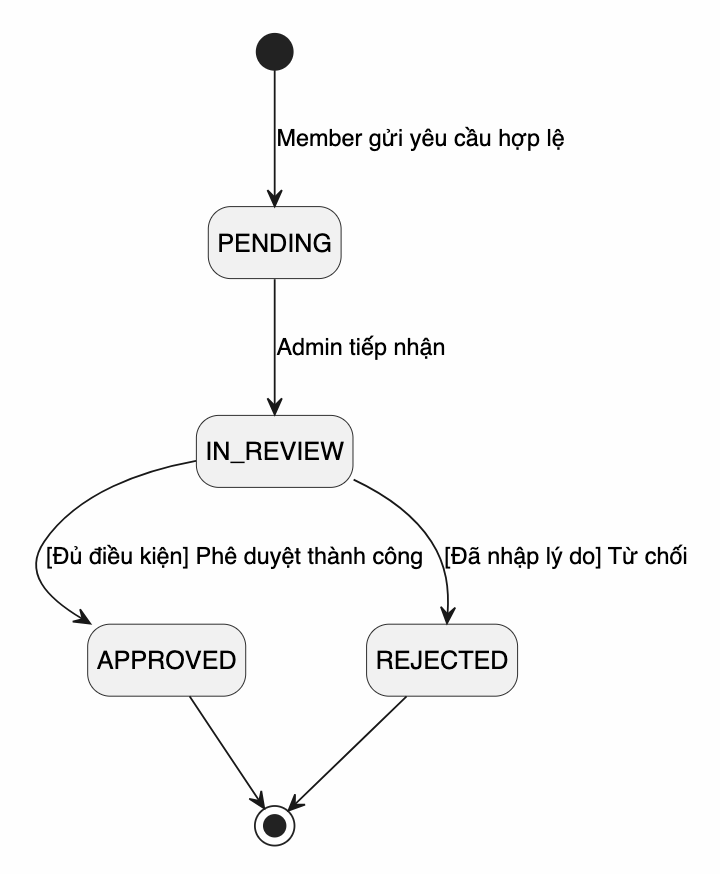
\includegraphics[width=\linewidth,height=100mm,keepaspectratio]{assets/chapter3/state-submission.png}
    \caption{Sơ đồ trạng thái đóng góp}\label{fig:chapter3-submission}
  \end{minipage}\hfill
  \begin{minipage}[b]{0.48\linewidth}\centering
    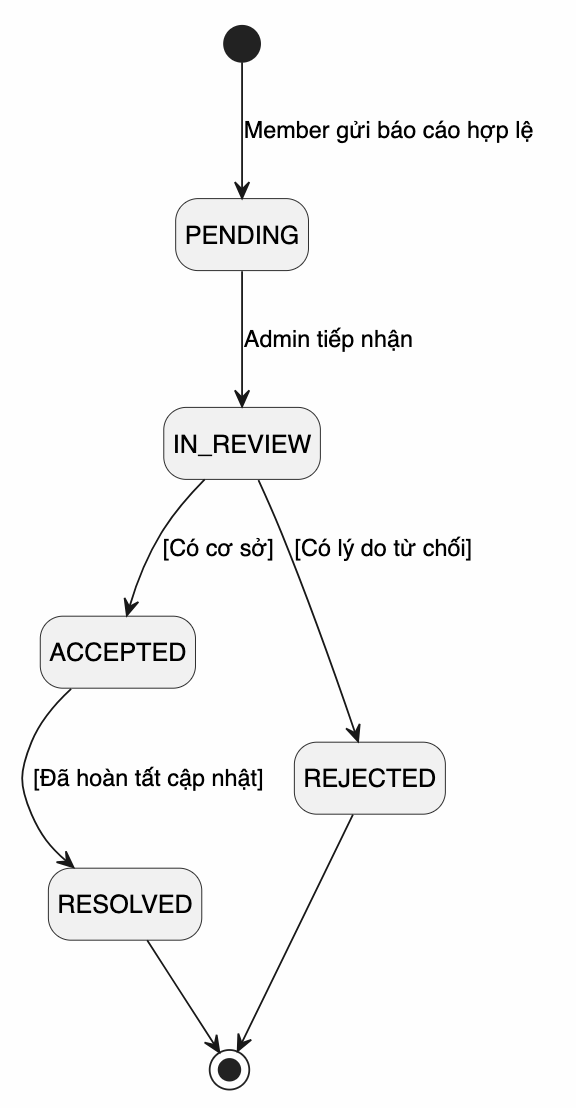
\includegraphics[width=\linewidth,height=100mm,keepaspectratio]{assets/chapter3/state-report.png}
    \caption{Sơ đồ trạng thái báo cáo}\label{fig:chapter3-report}
  \end{minipage}
\end{figure}

\begin{figure}[H]
  \centering
  \begin{minipage}[b]{0.48\linewidth}\centering
    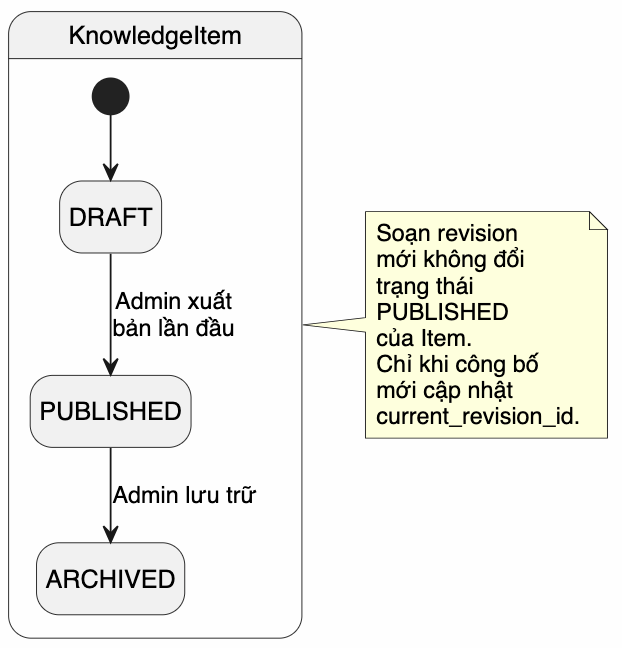
\includegraphics[width=\linewidth,height=73mm,keepaspectratio]{assets/chapter3/state-knowledge.png}
    \caption{Sơ đồ trạng thái tri thức}\label{fig:chapter3-knowledge}
  \end{minipage}\hfill
  \begin{minipage}[b]{0.48\linewidth}\centering
    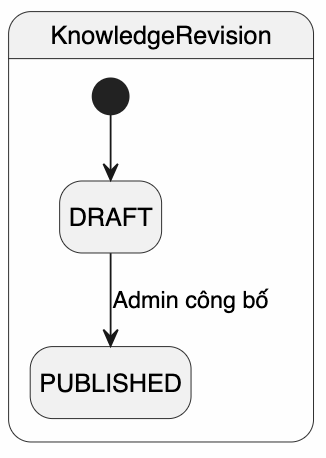
\includegraphics[width=\linewidth,height=73mm,keepaspectratio]{assets/chapter3/state-revision.png}
    \caption{Sơ đồ trạng thái phiên bản tri thức}\label{fig:chapter3-revision}
  \end{minipage}
\end{figure}

\subsection{Yêu cầu phi chức năng (NFR)}
Các ngưỡng là mục tiêu thiết kế đề xuất để nhóm xác nhận. Khi kiểm thử, ghi rõ máy chủ,
trình duyệt, kết nối mạng, quy mô dữ liệu và tải đồng thời.


\begin{longtable}{|L{18mm}|L{27mm}|L{94mm}|}
\caption{Yêu cầu phi chức năng}\label{tab:chapter3-nfr}\\\hline
\rowcolor{gray!15}\textbf{Mã} & \textbf{Thuộc tính} & \textbf{Yêu cầu và cách kiểm chứng}\\\hline
\endfirsthead
\hline
\rowcolor{gray!15}\textbf{Mã} & \textbf{Thuộc tính} & \textbf{Yêu cầu và cách kiểm chứng}\\\hline
\endhead
\endfoot
NFR-01 & Hiệu năng API & Mục tiêu p95 thời gian phản hồi API tìm kiếm, danh sách và chi tiết không vượt quá 2 giây với 20 yêu cầu đồng thời. Ghi rõ quy mô dữ liệu và môi trường đo.\\\hline
NFR-02 & Hiệu năng giao diện & Mục tiêu p95 từ khi mở trang khám phá đến khi bản đồ sẵn sàng chọn địa phương không vượt quá 3 giây. Ghi rõ thiết bị và mạng khi đo.\\\hline
NFR-03 & Dễ sử dụng & Từ bản đồ sẵn sàng, khách mở bài chi tiết trong tối đa ba thao tác chọn gồm địa phương, danh mục và bài. Luồng đọc mở công khai.\\\hline
NFR-04 & An toàn xác thực & Mật khẩu được băm bằng thuật toán dành cho mật khẩu trước khi lưu.\\\hline
NFR-05 & Bảo vệ phân quyền & Backend kiểm tra quyền và trạng thái tài khoản đối với mọi API có đặc quyền. Chỉ admin được gọi API duyệt hoặc xuất bản.\\\hline
NFR-06 & An toàn đầu vào & Kiểm tra và xử lý đầu vào để phòng XSS, SQL injection và tệp không hợp lệ. Giới hạn đề xuất là 5 ảnh, 5 MB mỗi ảnh và tối đa 5 lần gửi đóng góp hoặc báo cáo mỗi tài khoản trong 60 phút.\\\hline
NFR-07 & Toàn vẹn dữ liệu & Kiểm tra khả năng hoàn tác khi duyệt, xuất bản hoặc giải quyết báo cáo gặp lỗi, kể cả khi có thao tác đồng thời.\\\hline
NFR-08 & Truy vết & Tra cứu được lịch sử phiên bản, nguồn và quyết định kiểm chứng, gồm người xử lý và thời điểm.\\\hline
NFR-09 & Bảo trì & Chia mã thành các module có trách nhiệm rõ. Backend thực thi các kiểm tra quyền và quy tắc nghiệp vụ.\\\hline
NFR-10 & Mở rộng dữ liệu & Có thể bổ sung tỉnh/thành, danh mục và bài bằng dữ liệu cấu hình mà không đổi cấu trúc cốt lõi của CSDL.\\\hline
NFR-11 & Chất lượng nội dung & Bài công khai đạt checklist dữ liệu bắt buộc và có nguồn tham khảo. Ảnh công khai có thông tin xuất xứ và quyền sử dụng.\\\hline
NFR-12 & Tính sẵn sàng & Nếu có triển khai trực tuyến và giám sát, mục tiêu là ít nhất 99\% trong 7 ngày liên tục, không tính bảo trì đã thông báo. Nghiệm thu dựa trên số liệu đo.\\\hline
NFR-13 & Độ tin cậy & Thao tác lặp hoặc đồng thời trên một yêu cầu tạo tối đa một kết quả nghiệp vụ. Hệ thống chỉ ghi nhận hoàn tất sau khi giao dịch thành công.\\\hline
NFR-14 & Quyền riêng tư & Thành viên chỉ xem yêu cầu của mình. API công khai và nhật ký phải bảo vệ chứng cứ chưa công khai và dữ liệu tài khoản. Kiểm tra bằng truy cập chéo tài khoản.\\\hline
\end{longtable}

\ReportNeedSpace{50mm}
\subsection{Use case và đặc tả luồng chính}
\subsubsection{Danh sách use case và sơ đồ tổng quan}

\begingroup
\setlength{\extrarowheight}{0pt}
\begin{longtable}{|L{17mm}|L{64mm}|L{30mm}|L{23mm}|}
\caption{Danh sách use case}\label{tab:chapter3-usecases}\\\hline
\rowcolor{gray!15}\textbf{Mã} & \textbf{Use case} & \textbf{Tác nhân} & \textbf{FR liên quan}\\\hline
\endfirsthead
\hline
\rowcolor{gray!15}\textbf{Mã} & \textbf{Use case} & \textbf{Tác nhân} & \textbf{FR liên quan}\\\hline
\endhead
\endfoot
UC-01 & Tìm kiếm và khám phá theo địa phương, danh mục & Khách, thành viên & 01--07\\\hline
UC-02 & Đọc bài và xem nguồn tham khảo & Khách, thành viên & 08--09\\\hline
UC-03 & Gửi yêu cầu đóng góp tri thức mới & Thành viên & 11--13\\\hline
UC-04 & Báo cáo tri thức sai hoặc lỗi thời & Thành viên & 14--15\\\hline
UC-05 & Kiểm chứng và xử lý đóng góp & Admin & 17--20, 25, 32--34\\\hline
UC-06 & Kiểm chứng và xử lý báo cáo sai lệch & Admin & 17, 21--25, 32--34\\\hline
UC-07 & Quản lý kho tri thức và nguồn & Admin & 25--29\\\hline
UC-08 & Theo dõi kết quả yêu cầu đã gửi & Thành viên & 16\\\hline
UC-09 & Quản lý trạng thái tài khoản thành viên & Admin & 30\\\hline
UC-10 & Đăng ký, đăng nhập hoặc đăng xuất theo vai trò & Khách, thành viên, admin & 10, 31\\\hline
UC-11 & Hỏi đáp về bài đang đọc bằng RAG & Khách, thành viên & 35\\\hline
\end{longtable}
\endgroup

\begin{figure}[H]
  \centering
  \begin{minipage}[t]{0.52\linewidth}\centering\vspace{0pt}
    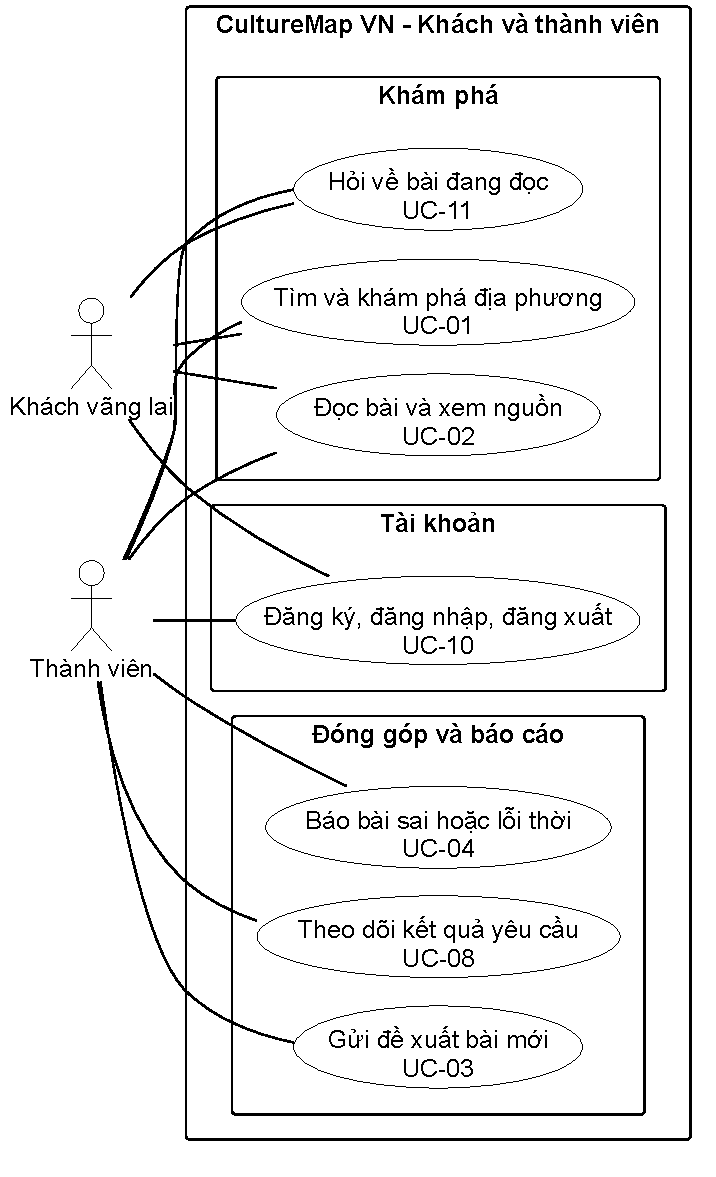
\includegraphics[width=\linewidth,height=130mm,keepaspectratio]{diagrams/output/chapter3-usecases.pdf}
  \end{minipage}\hfill
  \begin{minipage}[t]{0.45\linewidth}\centering\vspace{0pt}
    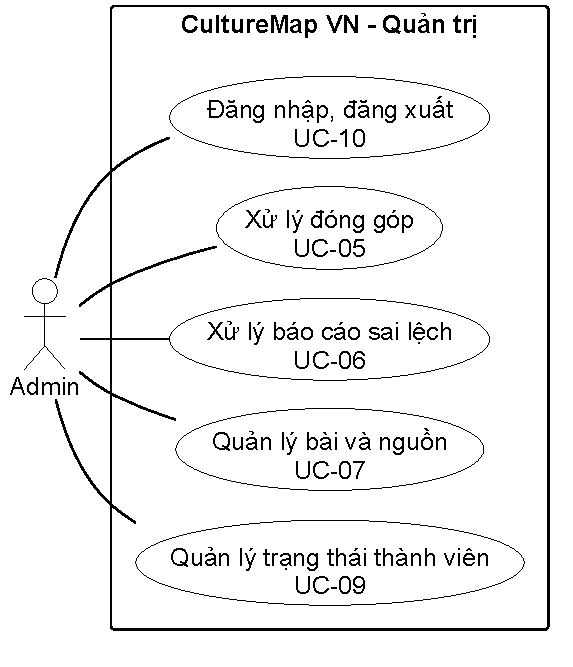
\includegraphics[width=\linewidth,height=130mm,keepaspectratio]{diagrams/output/chapter3-usecases-admin.pdf}
  \end{minipage}
  \caption{Sơ đồ tổng quan các use case CultureMap VN}
  \label{fig:chapter3-usecase}
\end{figure}

\subsubsection{Bảng đặc tả use case chính}
\par\noindent\mbox{}\par\vspace{2mm}

\ReportNeedSpace{186mm}
\subsection{Hoạt động và vòng đời nghiệp vụ}
\subsubsection{Luồng đóng góp tri thức mới}
\begin{figure}[H]
  \centering
  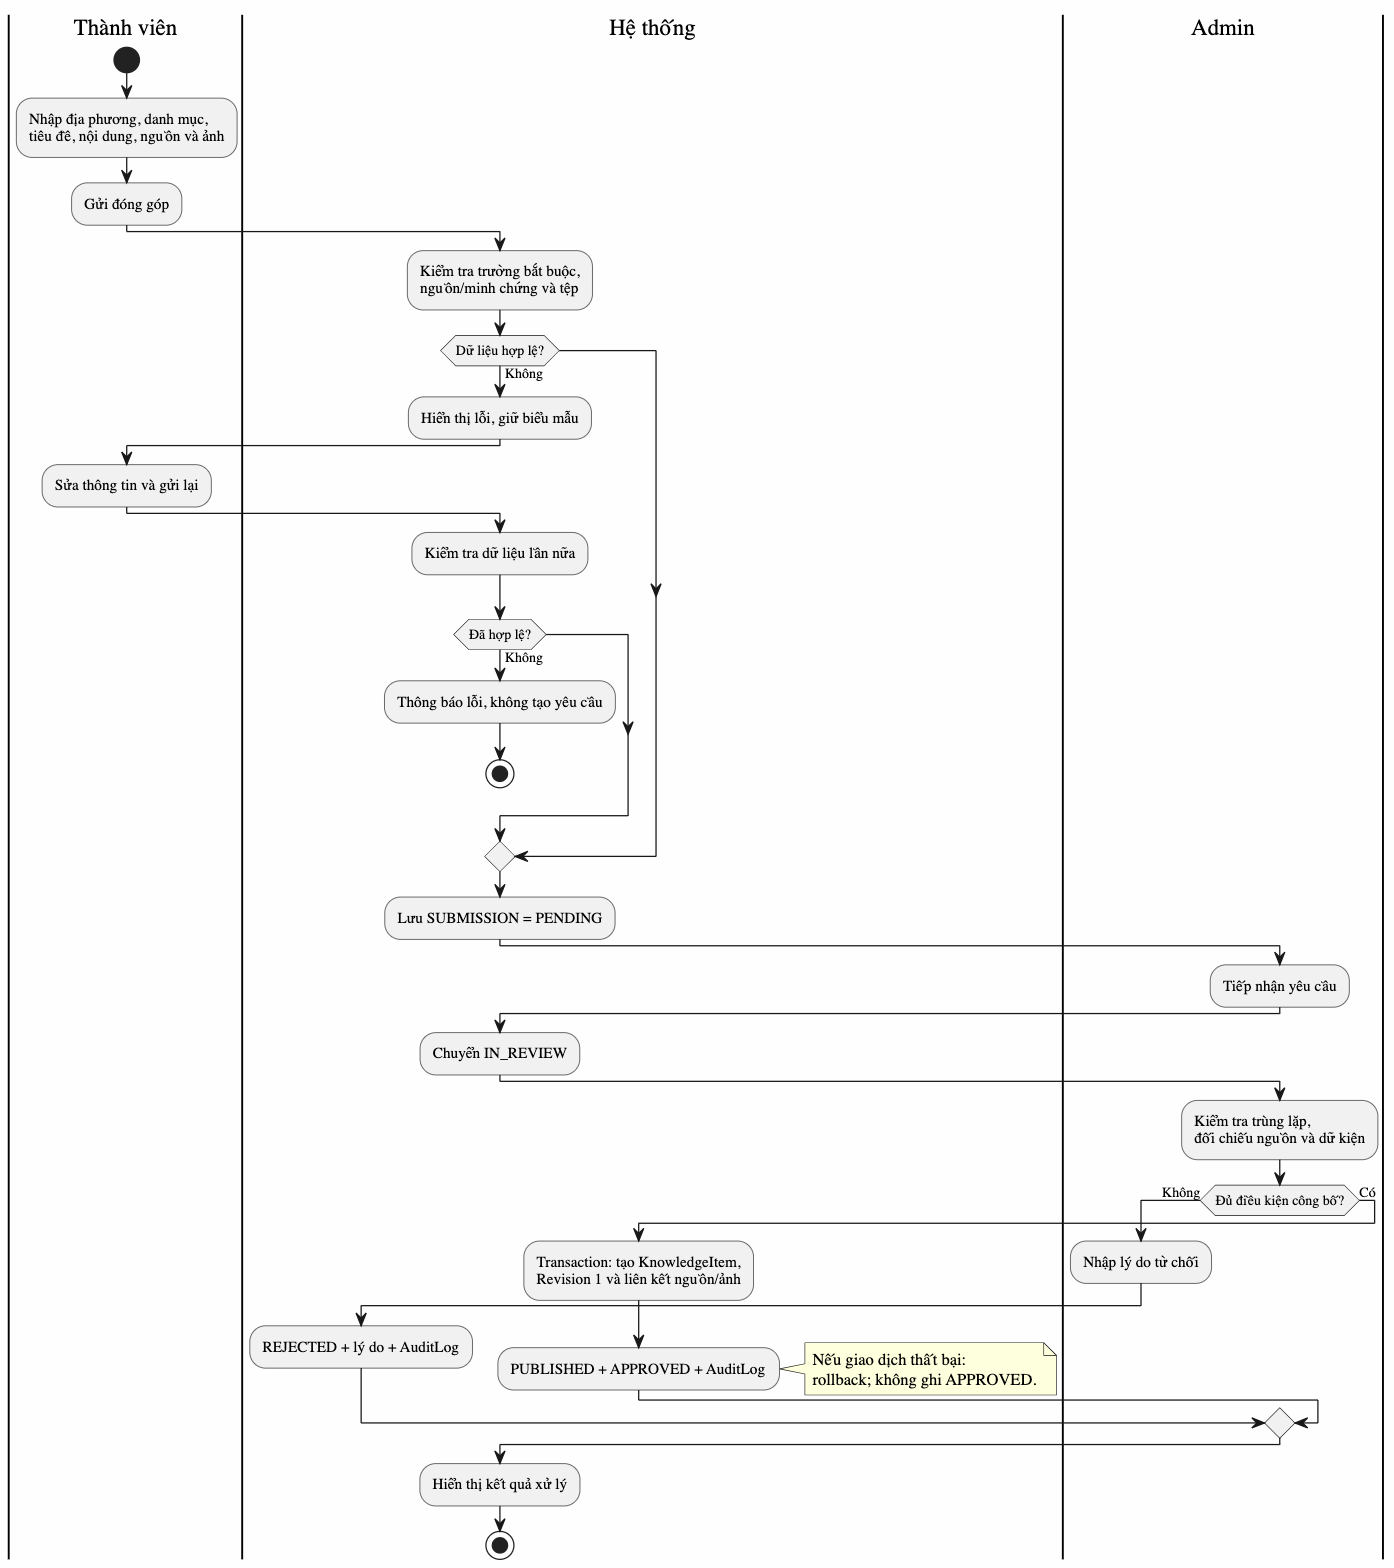
\includegraphics[width=\linewidth,height=160mm,keepaspectratio]{assets/chapter3/activity-submission.png}
  \caption{Quy trình tiếp nhận, kiểm chứng và công bố đóng góp}
  \label{fig:chapter3-activity-submission}
\end{figure}

\ReportNeedSpace{150mm}
\subsubsection{Luồng báo cáo và cập nhật tri thức}
\begin{figure}[H]
  \centering
  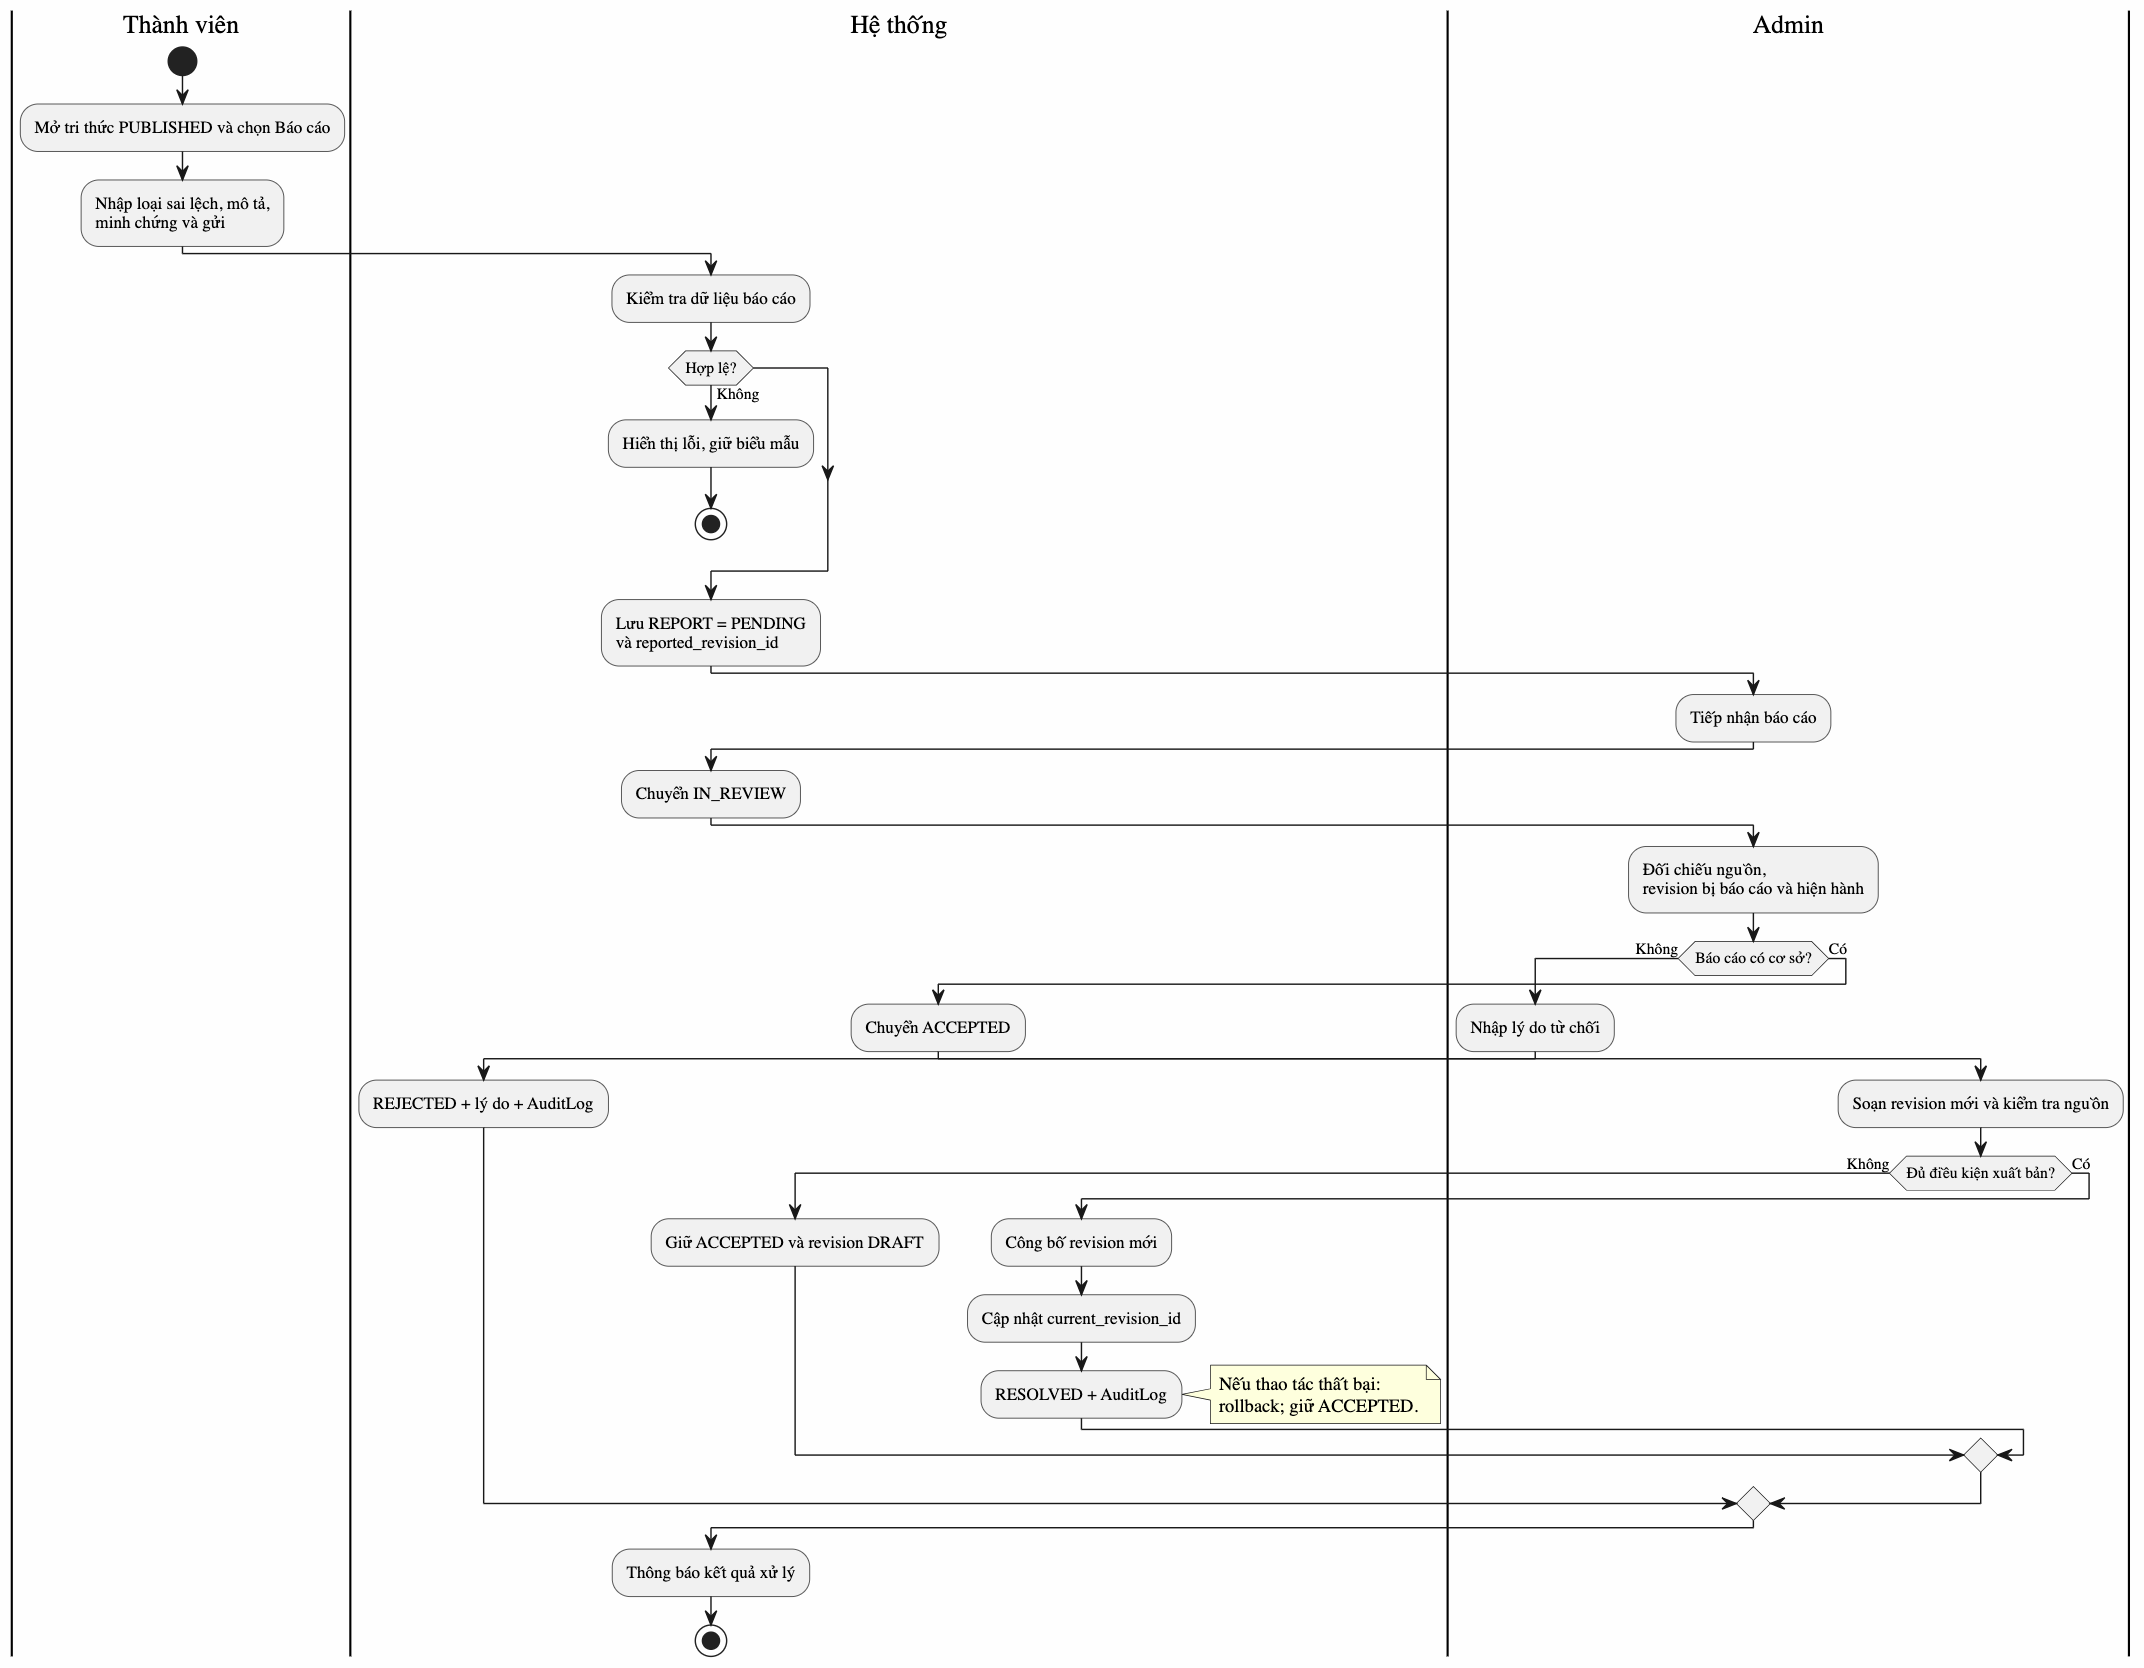
\includegraphics[width=\linewidth,height=152mm,keepaspectratio]{assets/chapter3/activity-report.png}
  \caption{Quy trình xác minh báo cáo sai lệch và tạo phiên bản mới}
  \label{fig:chapter3-activity-report}
\end{figure}
Duyệt đóng góp tạo một tri thức mới. Giải quyết báo cáo bằng chỉnh sửa tạo phiên bản mới
của tri thức đã có. Cả hai luồng lưu nguồn, người xử lý và nhật ký để đối chiếu.

\subsection{Truy vết yêu cầu}
\par\noindent\mbox{}\par\vspace{2mm}
\endgroup
